%%%
%%% prediction.tex
%%%

%\section{Route Prediction Algorithm}
%\label{sec:algos}


\section{Preliminaries}\label{sec:basic}

\begin{table}[t]
\begin{small}
\begin{center}
\begin{tabular}{|lp{4in}l|} \hline
{\em Symbol} & {\em Description} & {\em Section} \\
\hline
\multicolumn{3}{c}{{\sc Functions on Routes}} \\ \hline
$\lambda_r$ & Takes a set of routes received at router $r$ and outputs
the best route at router $r$, according  
to the BGP decision process applied at router $r$ & \ref{sec:basic} \\
$\gamma$ & Takes a set of routes and extracts the subset whose
attributes are equally good up through the first four steps of the 
decision process & \ref{sec:basic} \\
$\sigma$ & Takes a set of routes and extracts the subset whose
attributes are equally good up through the first {\em three} steps of the 
decision process & \ref{sec:fm_med} \\ 
\hline

\multicolumn{3}{c}{{\sc Sets of Routes or Routers (Initial Inputs)}} \\ \hline
$R$ & routers in the AS & \ref{sec:basic} \\
$A$ & routers that have been activated & \ref{sec:rr_nomed} \\ 
$E$ & eBGP-learned routes & \ref{sec:basic} \\
$E_r$ & eBGP-learned routes at router $r$ & \ref{sec:basic} \\
$N$ & number of eBGP-learned routes (\ie, $|E|$) & \ref{sec:basic} \\
\hline

\multicolumn{3}{c}{{\sc Sets of Routes (Intermediate and Final 
Outputs)}} \\ \hline
$I_r$ & iBGP-learned routes at router $r$ & \ref{sec:basic} \\
$P_r$ & All routes learned at router $r$ & \ref{sec:basic} \\
$b_r$ & The best route that router $r$ selects. & \ref{sec:basic}  \\ 
$C$ & The set of candidate routes at some intermediate activation. A
subset of $E$.& \ref{sec:simple} \\
$C_r$ & The set of candidate routes at router $r$ at some intermediate
activation. A subset of $E_r$.& \ref{sec:fm_med} \\
$B$ & The set of best routes computed by the algorithm.  A subset of
$C$. & \ref{sec:simple} \\
$L$ & The set of routes eliminated at some activation step. &
\ref{sec:fm_med} \\
\hline


\multicolumn{3}{c}{{\sc iBGP Topology}} \\ \hline
$S$ & iBGP sessions. & \ref{sec:rr_nomed} \\
$G$ & iBGP session graph. $G = (R,S)$. & \ref{sec:rr_nomed} \\
\hline

\end{tabular}
\end{center}
\end{small}
\caption{Description of the notation used in this chapter, and the
  sections where each piece of notation is introduced.}
\label{tab:notation}
\end{table}


%Computing the effects of the BGP decision
%process, iBGP route propagation, and IGP path computation for
%each router in the AS is challenging.  
% Sets E and I
We first introduce some notation.  Table~\ref{tab:notation} lists
the notation we use for the remainder of this chapter and summarizes
where this notation is introduced.  We assume that the AS has a set of
$N$ eBGP-learned routes, $E$, for a given destination prefix, which it
learns at $R$ routers.  $E$ contains the eBGP-learned routes after each
router in the AS has applied its local import policy (which may filter
some set of the routes it receives and set or modify the route
attributes of others).  For convenience, we define $E_r \subseteq E$ as
the set of eBGP-learned routes at router $r\in R$.  At any given time, a
router $r$ also has zero or more iBGP-learned routes $I_r \subseteq E$.
% decision process
We define two useful functions:
\begin{itemize}
\itemsep=-1pt
\item $\lambda_r$, which takes a set of routes at router $r$ and
  produces the best route at router $r$ according to the BGP decision
  process in Table~\ref{tab:background:decision}.  The subscript on
  $\lambda_r$ is necessary because different routers can apply the BGP
  decision process to the same set of routes and obtain different
  results based on the BGP session from which they learn the route and
  their location in the topology.  For example, in
  Figure~\ref{fig:example}, router $X$ would treat the route learned
  from AS $B$ as an eBGP-learned route with the router ID of the eBGP
  session with $B$. On the other hand, $Z$ sees an iBGP-learned route
  with an IGP path cost of $2$ and the router ID associated with the
  iBGP session to $X$.

\item $\gamma$, which takes a set of BGP routes, $C$, and produces $C'
  \subseteq C$, such that routes in $C'$ are the network-wide best
  routes based on the first four steps in
  Table~\ref{tab:background:decision}.

  Unlike $\lambda_r$, $\gamma$ has {\em global} (\ie, network-wide)
  context; that is, its context is not router-specific.  When the
  routers' selection functions do not satisfy determinism, each router's
  best route is not guaranteed to be in the set $\cup_r \lambda_r(E_r)$.
  In Sections~\ref{sec:med_model} and~\ref{sec:best_egress}, we will
  apply $\gamma$ to a set of routes when it is safe to eliminate all
  routes that could {\em never} be the best route at any router.  In
  these sections, we will see that as long as all routers have either
  complete visibility of the routes that the AS learns via eBGP or
  selection functions that satisfy determinism, every router will
  ultimately select a route from $\gamma(E)$.
\end{itemize}


\section{Simple Case: BGP with Determinism and Full Visibility }
\label{sec:egress_set}
\label{sec:simple}

In this section, we describe an algorithm that predicts the outcome of
BGP route selection 
when a network employs a full mesh iBGP topology and the MED attribute
is compared across all routes (which we also refer to as ``no MED'' or
``without MED'').  This algorithm works as long as routers compare the
MED attribute across all candidate routes and when the network does not
use route reflection.  This scenario may be the case for many small stub
ASes that do not have customers of their own: a network that does not
have many routers will typically configure its iBGP topology as a full
mesh, and a stub AS typically does not receive (or honor) MEDs from the
ASes from which it buys transit.  In practice, some transit ISPs even
configure their routers to compare the MED attribute across all
candidate routes (often to avoid problems with oscillation), and most
small networks do not use route reflection.

After describing the route prediction algorithm and proving its
correctness, we explain 
two basic properties that hold in this case that make the prediction
algorithm quite simple and explain why two artifacts of BGP---MED and
route reflection---can cause these properties to be violated.

A full mesh iBGP topology provides full visibility of BGP routes at each
router: every router learns the set of routes selected by every
eBGP-speaking router in the AS.
Furthermore, when the MED attribute is compared across all routes (as
opposed to just those from the same neighboring AS) a router's ranking
over the set of routes it learns form a total ordering, which implies
that the first condition of determinism
(Definition~\ref{def:determinism}) is satisfied.
% (\ie, $\forall P'_r \subseteq P_r$, if $a\in P'_r \subseteq
%P_r$ and $\lambda_r(P_r) = a$, then $\lambda_r(P'_r) = a$).  
These characteristics allow us to devise a relatively simple algorithm
to compute the outcome of BGP route selection at each router in the AS.


\begin{figure}
\centering{\em Algorithm: Full Mesh, No MED} \\
\centering\framebox{
\begin{minipage}{4in}
\begin{tabbing}
\hspace*{0.5cm}\=\hspace{0.5cm}\=\hspace{0.5cm}\=\hspace{0.3cm}\=
\hspace{0.3cm}\=\hspace{0.3cm}\=\hspace{0.3cm}\=\hspace{0.3cm}\=\kill
{\sc SelectBest\_eBGP}($E$, $R$)\\
\> {\em // Build the set of locally best routes at each router.} \\
\> {\em // This set is the set of candidate best eBGP routes.} \\
%%\>\> $b_r \leftarrow \lambda_r(E_r)$ \\
\> $C \leftarrow \cup_r \lambda_r(E_r)$\\
\\
\> {\em // Eliminate all routes from C that } \\
\> {\em // do not have highest local preference,} \\
\> {\em // shortest AS path length, lowest origin type, lowest MED} \\
\> $B \leftarrow \gamma(C)$ 
\end{tabbing}
\end{minipage}
}
\caption[Algorithm: Full Mesh, No MED]{Algorithm for computing the best
  route at eBGP 
  routers, assuming that MED is compared across all routes (\ie, that
  there exists a total ordering of routes at each router).}
\label{fig:b2_tot_order}
\end{figure}

In this case, the algorithm for computing the best route at every
eBGP-speaking router is shown in Figure~\ref{fig:b2_tot_order}.  The
algorithm takes as input the set of all eBGP-learned routes, $E$, and
the set of all eBGP-speaking routers, $R$, and produces the set of best
eBGP routes, $B$. $E_r$ refers to all eBGP-learned routes learned by
router $r$, and $C$ represents the set of candidate routes after each
router selects the best route from the set of its eBGP-learned routes.
The output of this algorithm is $B = \gamma(C)$, the set of all best
routes to this destination, such that $b_r = \lambda_r(B)$.  The
algorithm proceeds in two steps. The first step computes the locally
best BGP route at each eBGP-speaking router; this step guarantees that
each router selects no more than one eBGP-learned route.  The second
step eliminates any route from this set for which a router would select
another router's iBGP route over its own locally best route.

The first step of the algorithm scans all $N$ eBGP-learned routes and
selects the best eBGP-learned route at each router, if any; at most
$|R|$ routes remain after this step.  The second step selects, for each
router $r \in R$, the best route from $R$.  Thus, the running time will
be $O(N + |R|^2)$, where $N$ is the number of eBGP-learned routes, and
$|R|$ is the number of routers in the system (a full mesh iBGP
configuration will have $|R|(|R|-1)$ iBGP sessions).  When $|R|>N$, the
$N$ term is dominated, so the running time is $O(|R|^2)$.  When $N>|R|$,
however, a simpler approach to the algorithm would simply be to apply
$\lambda_r(E)$ at each router, which has $O(N|R|)$ running time.  Thus,
the computational complexity for route prediction is proportional to the
total number of routes in the system.

To prove that this algorithm is correct, we must show that this
algorithm accurately emulates {\em one} activation sequence;
Observation~\ref{t:order} guarantees that as long as the algorithm
correctly emulates some activation, it will correctly emulate BGP
route selection. 

\begin{theorem}\label{t:ebgp_to}
When each router can produce a total ordering over all possible
candidate routes, the algorithm in Figure~\ref{fig:b2_tot_order}
correctly computes the outcome of the decision process 
for all routers that select an eBGP-learned route as their best
route.
\end{theorem}

\vspace*{0.1in}
\begin{proof}
We prove this theorem constructively, by showing that the algorithm
correctly emulates an activation sequence and message ordering that
could occur in BGP.  Consider the following ordering:
\begin{enumerate}
\itemsep=-1pt
\item All routers receive routes to the destination via eBGP.
Then, every router is activated simultaneously.
\item Every router advertises its locally best route via iBGP.  
  After all iBGP messages have been exchanged, every router is 
activated simultaneously.
\end{enumerate}

In the first phase, each router $r$ computes $\lambda_r(E_r)$, resulting
in a set of candidate routes $C = \cup_r \lambda_r(E_r)$, as in the
first line of the algorithm in Figure~\ref{fig:b2_tot_order}.  Then,
each router learns these routes.
%, resulting in $P_r=C$ for all $r\in R$.
Note that $B \subseteq C$ by definition, which means that each router
that learns a route to the destination via eBGP has either zero or one
route in $B$.  We consider both cases.
%
If a router $r$ has a route in $C$ but not in $B$, then $r$'s
eBGP-learned route $b_r=\lambda_r(E_r)$ must have been worse according to the first
four steps of the decision process than some other route, $b_s=\lambda_s(E_s)$ in $C$
(otherwise, $\gamma(C)$ would not have eliminated it).  But in a
full mesh iBGP topology, $r$ would learn
a route via iBGP that is at least as good as $b_s$, so $b_r$ would also be
eliminated in phase~2 of the activation.
%
Of course, if a router has a route in $C$, then that must be the route
that it would select after phase~2 of activation: it is equally good as
all routes in $\gamma(C)$ through the first 4 steps of the decision
process (by construction), and it prefers its own best route over any
iBGP-learned route (by step~5 of the decision process).
\end{proof}

\begin{table}[t]
\begin{center}
\begin{small}
\begin{tabular}{r|cc|ccc}
$\S$ & {\em MED} & {\em RR} & {\em Running Time} & Prop.~\ref{l:c1}
  & Prop.~\ref{l:c2} \\ \hline 
\ref{sec:simple} & No & No & $O(N+|R|^2)$ & $\bullet$ & $\bullet$ \\ 
\ref{sec:fm_med} &Yes & No & $O(N \log N+ N|R|)$ &  & $\bullet$ \\ 
\ref{sec:rr_nomed} &No & Yes & $O(N+|S|)$ & $\bullet$ & $\bullet$  \\ 
\ref{sec:rr_med} &Yes & Yes & $O(N \log N + N|R| + N|S|)$ & &  \\ 
\end{tabular}
\end{small}
\end{center}
\caption{Properties of the BGP route prediction algorithms in each of the four
  cases (with and without MED, and with and without route reflection).} 
\label{tab:runningtimes}
\end{table}

This simple algorithm works because two properties hold.  First, when
MED is compared across all routes, every router that selects a route
from the set of eBGP-learned routes will select its locally best route.
Second, when the iBGP topology is a full mesh, each BGP-speaking router
ultimately selects a route in $\gamma(E)$; that is, every router
ultimately selects a route that has the maximum local preference,
minimum AS path length, lowest origin type, and lowest MED (assuming
MEDs are compared across all routes).  Table~\ref{tab:runningtimes}
summarizes when these two properties hold, for all
possible combinations of MED and route reflection (the rest of this
section treats defines these two properties more formally).  The table also
indicates the computational complexity for computing the best route at
each router, for each scenario.  We now formalize these two properties,
explain why they make route prediction simple, and present cases where
BGP violates each of them.


\subsection{Property \#1: Every best route is some router's
  best eBGP route.}

This property holds only if every router's selection function satisfies
determinism.  We now formalize this property, prove that determinism
is required to ensure that it holds, and show an example where this
property is violated if BGP does not satisfy determinism.


\begin{property}\label{l:c1}
If determinism is satisfied, then each router
ultimately either selects its own best eBGP-learned route or some
iBGP-learned route.  Formally, $b_r \in E_r \Rightarrow b_r =
\lambda_r(E_r)$.
\end{property}
\vspace*{0.1in}
\begin{proof}
By definition, each router $r$ applies the route selection process to the union
of the routes it learns via eBGP and iBGP: $b_r = \lambda_r(E_r \cup
I_r)$. Therefore, either $b_r \in E_r$ or $b_r \in I_r$.  Furthermore,
because the first condition of determinism is satisfied, the router $r$'s
preferences over routes in $E_r \cup I_r$ form a total ordering, so
either $b_r = \lambda_r(E_r)$ or $b_r = \lambda_r(I_r)$.  But, if $b_r
\neq \lambda_r(E_r)$, then $b_r = \lambda_r(I_r)$, so $b_r\in I_r$ and
$b_r \not\in E_r$.
%Because step~5
%of the BGP decision process prefers routes in $E_r$ over routes in
%$I_r$, if $b_r \in E_r$, then, by definition, $b_r \in \lambda(E_r)$.
\end{proof}

\noindent
Property~\ref{l:c1} makes it possible to propagate the effects of route
selection at each router only once, because each router ultimately selects
its locally best eBGP-learned route or some other router's locally best route.


\begin{figure}[t]
\begin{center}
\begin{psfrags}
\psfrag{R_1}{{\Large $R_1$}}
\psfrag{R_2}{{\Large $R_2$}}
\psfrag{a}{{\Large $a$}}
\psfrag{b}{{\Large $b$}}
\psfrag{c}{{\Large $c$}}
\resizebox{0.7\textwidth}{!}{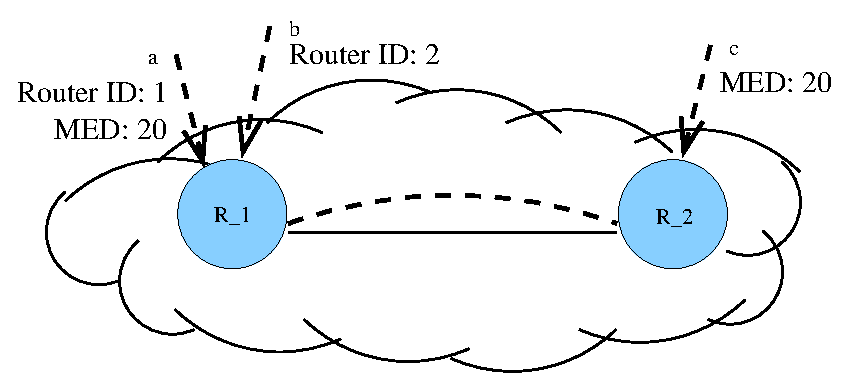
\includegraphics{sandbox/figures/med_counterex.eps}} 
\end{psfrags}
\end{center}
\caption[With MED, a router may select a route that is no
  router's best eBGP route.]{With MED, a router may select a route that is no
  router's best eBGP route, thus violating Property~\ref{l:c1}.}
\label{fig:med_counterex}
\end{figure}

Unfortunately, when the MED attribute is only compared among routes from
the same AS, BGP does not satisfy determinism, so this property no
longer holds.  Figure~\ref{fig:med_counterex} shows an example where
this property is violated.  In this example, router $R_1$'s ranking
between $a$ and $b$ depends on whether it learns route $c$.  Thus, even
though route $a$ is $R_1$'s locally best route (by the router ID
tiebreak), $R_2$ ultimately selects route $b$ ($c$ eliminates $a$ due to
MED due to MED, and $R_1$ selects $b$ over $a$ because $b$ is learned
via eBGP), which is {\em no} router's best eBGP route.  As such, the
simple algorithm that selects each router's best route from the set of
best eBGP routes does not work: a na\"{i}ve algorithm would result in
precisely the ``back and forth'' behavior described in
Section~\ref{sec:sb_challenges}.  Section~\ref{sec:med_model} describes an
alternate route prediction algorithm that handles this case.


\subsection{Property \#2: Every best route is in $\gamma(E)$.}

This property states that every router selects a route that is equally
good up through the MED comparison step of the decision process.
Intuitively, it might seem that this property would always hold---why
would a router ever select a route with a lower local preference, longer
AS path, higher origin type, or higher MED value if it had a better
route available?  In fact, in certain iBGP configurations, a route
reflector can prevent a router from {\em learning} an eBGP-learned route with
a lower MED value than the one it selects.  Property~\ref{l:c2} holds if either
the iBGP topology is a full mesh or determinism is satisfied.  We now
formally state the conditions when this property holds, show an
example where a BGP configuration can violate this property, and briefly
discuss its implications for route prediction.

\begin{property}\label{l:c2}
If (1)~every router in the AS receives the best eBGP-learned route from
every other router in the AS or (2)~all route attributes are compared
across all routes (\ie, it is possible to construct a total ordering
over all routes) and every router receives at least one route in
$\gamma(E)$, then every router $r$ will ultimately select a route, $b_r
\in \gamma(E)$, where $E$ is the set of all eBGP-learned routes.
\end{property}
\vspace*{0.1in}
\begin{proof}
Define $P_r \subseteq E$, the set of routes that router $r$ learns (\ie,
$P_r = E_r \cup I_r$).  Assume that some router $r$ selects $b_r =
\lambda_r(P_r) \notin \gamma(E)$.  This property implies that $P_r\cap
\gamma(E) = \phi$ (\ie, that $P_r$ contains {\em no} routes in
$\gamma(E)$; otherwise, $b_r$ would be better than all routes in
$\gamma(E)$, which contradicts the definition of $\gamma$.  But, if $P_r
\cap \gamma(E) = \phi$, then the iBGP topology is such that $r$ does not
learn all routes, because at least one router $s \in R$ selects a route
from $\gamma(E)$, and router $r$ would have learned that route from $s$.
If path visibility is satisfied and $b_r \not\in \gamma(E)$, this also
implies that some route attribute is not compared across all routes
(\ie, it is not possible to form a total ordering): otherwise, given a
total ordering, if one router selects a route from $\gamma(E)$, then every
router either learns that route and selects it, or selects its own route
(which must be in $\gamma(E)$, by total ordering) and propagates that
route.
\end{proof}

\noindent
Property~\ref{l:c2} makes it possible to compute the route that each
router $r$ selects by applying $\lambda_r$ to the set of {\em all}
locally best routes, $B$ (\ie, $b_r = \lambda_r(B)$), thus eliminating
other routes.

Unfortunately, this property is not guaranteed when determinism is
violated and every router does not learn every eBGP-learned route.
Consider the example shown in Figure~\ref{fig:ibgp2}.  The network
learns routes to some destination at routers $X$, $Y$, and $Z$ that are
equally good up to MED comparison. All three routers are clients of the
route reflector $RR$.  The routes at $X$ and $Y$ are learned from the
same next-hop AS, and $r_Y$ has a lower MED value.  One might think that
router $X$ would never select route $a$, since, after all, it has a
higher MED value than route $b$, but that is not the case in this
figure: $RR$ learns routes $a$, $b$, and $c$, and selects route $c$ as
its best route, because $c$ has the shortest IGP path cost.  As a
result, $X$ never learns route $b$.

When Property~\ref{l:c2} is not satisfied, route prediction must
essentially resort to simulation.  The problem in this case is that it
is impossible to know when activating any given router that it is safe
to eliminate {\em any} route that it learns via eBGP.  We discuss this
problem in more detail in Section~\ref{sec:best_egress}.

\begin{figure}[t]
\begin{center}
\begin{psfrags}
\psfrag{a}{{\Large $a$}}
\psfrag{b}{{\Large $b$}}
\psfrag{c}{{\Large $c$}}
\psfrag{RR}{{\LARGE $RR$}}
\psfrag{W}{{\LARGE $W$}}
\psfrag{X}{{\LARGE $X$}}
\psfrag{Y}{{\LARGE $Y$}}
\psfrag{Z}{{\LARGE $Z$}}
\resizebox{0.5\linewidth}{!}{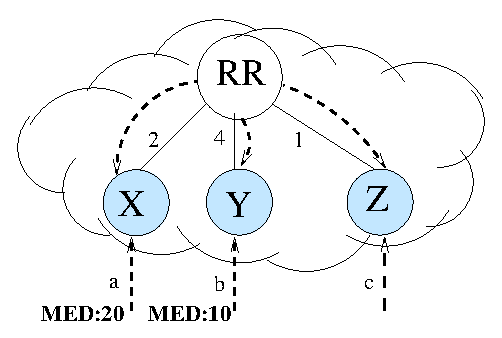
\includegraphics{sandbox/figures/ibgp2.eps}}
\end{psfrags}
\end{center}
\caption{When an AS's iBGP topology uses route reflectors and MED, a
  router may not always select a route in $\gamma(E)$. }
\label{fig:ibgp2}
\end{figure}




%This property also holds when the iBGP topology does not form a full
%mesh, as long as the MED attribute is compared across all routes, as
%discussed in more detail later in Section~\ref{sec:best_egress}.
%In the following subsection, we
%describe how these assumptions simplify modeling and 
%present an algorithm that models the outcome of the BGP decision
%process in the simple case of a full mesh iBGP topology where the MED
%attribute is compared across all routes, independent of the next-hop
%AS.
% (we assume in the next section that the MED
%attribute is compared across {\em all} routes).

%But, if $\lambda_r(P_r) \not\in
%\gamma(E)$, then all routes in $P_r \cap \gamma(E)$ must be worse in the first
%four steps of the decision process than $\lambda_r(P_r)$ and, hence, that
%all routes in $\gamma(E)$ are worse in first four steps than
%$\lambda_r(P_r)$.  But, since $\lambda_r(P_r) \not\in \gamma(E)$, this
%implies that $P_r \cap E = \phi$, which is a contradiction, since $P_r
%\subset E$ as long as the iBGP configuration forms a full mesh.
%








%%%%%%%%%%%%%%%%%%%%%%%%%%%%%%%%%%%%%%%%%%%%%%%%%%%%%%%%%%%%

\section{Route Computation without Determinism}\label{sec:med_model}

In this section, we present how to model path selection when the MED
attribute is compared only across routes learned from the same AS,
rather than across all routes for a destination prefix.  MED prevents
each router from having a total ordering over all possible candidate
routes, so it is actually possible to have $b_r \in E_r$ without $b_r =
\lambda_r(E_r)$.  In Section~\ref{sec:med}, we describe this problem in
more detail and describe why the simple approach presented in
Section~\ref{sec:simple} fails; then, we present an algorithm that
accurately computes the outcome of BGP path selection when MED is
compared only across routes from the same AS.

\subsection{Problems Introduced by MED}\label{sec:med}

The algorithm from Section~\ref{sec:simple} assumes that each router's
ranking between two routes is independent of whether other routes are
present (\ie, $\lambda_r(\{a,b\}) = a \Rightarrow \lambda_r(\{a,b,c\})
\neq b, \;\forall a,b,c$).  When MED is only compared across routes from
the same AS, the algorithm cannot simply select the locally best route
at each router, because a router may ultimately select a best route that
it learned via eBGP that was not its locally best route.
%$b_r \in E_r \not\Rightarrow b_r =
%\lambda_r(E_r)$.
%
This point has serious implications, because we can no longer assume
that if a router selects an eBGP-learned route to a destination, that
eBGP-learned route will be that router's locally best route; rather, the
route that the router ultimately selects may be worse than the ``best''
route at that router when compared only against routes learned via eBGP
at that router.  Thus, the approach from Section~\ref{sec:simple}, which
computes $b_r$ by taking the locally best route at each router from
$\gamma(E)$, may not compute the correct result.  Using the example
in Figure~\ref{fig:med}, we explain why two seemingly-natural
approaches to computing the routes do not work:

%This complication arises because the BGP decision process
%only compares MED values for routes with the {\em same next-hop AS\/}.
%As such, the MED value of an eBGP route learned at one router may affect
%the {\em local\/} ranking of eBGP-learned routes at another router.

\begin{itemize}
\item {\em Local route elimination is not correct.}  The algorithm in
Figure~\ref{fig:b2_tot_order} would first apply $\lambda_r(E_r)$ at each
router.  In Figure~\ref{fig:med}, given the choice between the two
eBGP-learned routes $a$ and $c$, router $X$ prefers $c$, because $c$ has
a smaller router ID.  Between routes $a$, $c$, and $d$ (which it learns
via $Y$), however, router $X$ prefers route $a$, because route $d$
eliminates route $c$ due to its lower MED value.  Thus, router $X$'s
preference between routes $a$ and $b$ depends on which route $Y$
selects.  The algorithm in Figure~\ref{fig:b2_tot_order} would compute
$\lambda_X(\{a,c\})=c$ and $\lambda_Y(\{b,d\})=d$ (resulting in
$C=\{c,d\}$), and ultimately compute $B=\{d\}$ because $d$ has a smaller
MED value than $c$.  In reality, though, router $X$ would select route
$a$ over $d$, because $a$ is an eBGP-learned route from a different
neighboring AS.

%One possible approach
%would be to select a best route {\em locally} at each router
%and
%subsequently eliminate routes from this set by comparing routes within
%this set of locally best routes (\ie, applying $\lambda_r(E_r)$ at each
%router and subsequently applying $\gamma$ to the remaining routes, as in
%the algorithm from Figure~\ref{fig:b2_tot_order}).   This approach does
%not work.
%
%Consider Figure~\ref{fig:med} and assume
%that AS 3 learns eBGP routes $\{a,b,c,d\}$ that are equally good through
%the first four steps of the BGP decision process.  Routes $a$ and $b$
%are learned 
%from AS 1, and routes $c$ and $d$ are learned from AS 2.
%
%With this approach, router $X$ selects route
%$c$ because its router ID is lower than that of $a$; similarly, router
%$Y$ selects route $d$.  This suggests that (after applying $\gamma$ to
%the remaining candidate routes) router $X$ would ultimately select $d$
%as its best route, since $d$ is better than $c$ due to MED comparison.
%This conclusion is incorrect, because $X$ will always prefer
%route $a$ over route $d$.  Essentially, the interaction between MED and
%router ID make it impossible to guarantee that route that a router
%ultimately selects as its best route will be from the set of locally
%best routes at each router.

%\subsubsection{Strawman 2: Global Route Elimination}\label{sec:sm2}

\item {\em Global route elimination is not correct.}
%Comparing all of the eBGP-learned routes {\em globally} (\ie,
%without regard to which router originally learned a route) to determine 
%the best route at a particular router is not correct.  
It might also seem reasonable to apply $\gamma$ globally, followed by
applying $\lambda_r$ locally at each router.
%Consider the example in Figure~\ref{fig:med}.
%
In Figure~\ref{fig:med}, a global comparison of 
the routes (\ie, applying $\gamma(\{a,b,c,d\})$), would first eliminate
$a$ and $c$ based on MED, and then   
router $X$ would select route $d$ (because $d$ is preferred to $b$ based on
the router ID comparison applied at router $Y$).   
%J i'm confused about b vs. d based on router-id -- doesn't the iBGP
%J session from Y have a single router-id that is the same for both
%J of these routes?
This conclusion is
incorrect, because $X$ would {\em always\/} prefer route $a$ over route $d$,
because $a$ is learned via eBGP (step 5) and $a$ and $d$ are equally good
up through step 4 (recall that a router does not compare the MEDs of routes
with different next-hop ASes).
\end{itemize}

\noindent
The crux of the problem is that the MED attribute makes it impossible to
produce an ordering of the routes at $X$ that is independent of the
presence or absence of other routes.

\begin{figure}[t]
\begin{center}
\begin{psfrags}
\psfrag{X}{{\Large $X$}}
\psfrag{Y}{{\Large $Y$}}
\psfrag{a}{$a$}
\psfrag{b}{$b$}
\psfrag{c}{$c$}
\psfrag{d}{$d$}
\resizebox{0.9\textwidth}{!}{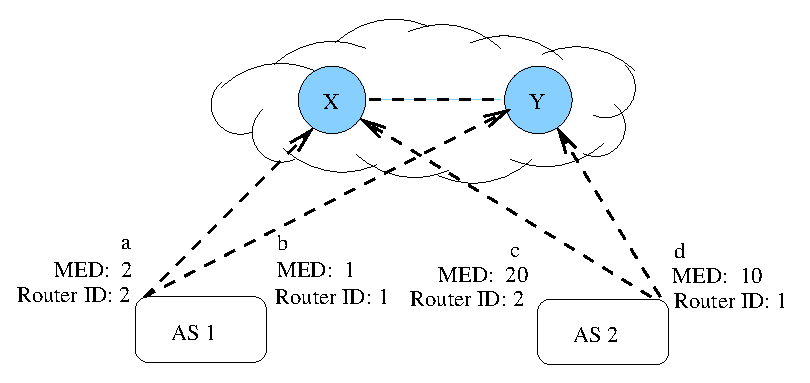
\includegraphics{sandbox/figures/med3.eps}}
\end{psfrags}
\end{center}
\caption[Interaction between MED and router ID in the BGP route selection
  process.]{Interaction between MED and router ID in the BGP route selection
  process.  $X$ and $Y$ are routers, each with direct eBGP sessions to
  ASes~$1$ and~$2$. $a$, $b$, $c$, and $d$ are routes learned via eBGP.}
\label{fig:med}
\end{figure}

%% Thus, the route prediction algorithm {\em must} take
%% into consideration the ranking of routes at each router, but, because of
%% the interactions between MED and router ID, it must eliminate suboptimal
%% routes in a way that actually emulates some specific message ordering.



\subsection{Algorithm: Full Mesh, MED}\label{sec:fm_med}


\begin{figure}
\centering{\em Algorithm: Full Mesh, MED} \\
\centering\framebox{
\begin{minipage}{4in}
\begin{tabbing}
\hspace*{0.5cm}\=\hspace{0.5cm}\=\hspace{0.5cm}\=\hspace{0.3cm}\=
\hspace{0.3cm}\=\hspace{0.3cm}\=\hspace{0.3cm}\=\hspace{0.3cm}\=\kill
{\sc SelectBest\_eBGP\_MED}($E$, $R$)\\
\> {\em // Eliminate all routes from C that } \\
\> {\em // do not have highest local preference,} \\
\> {\em // shortest AS path length, lowest origin type} \\
\> $C \leftarrow \sigma(E)$ \\
\> $B_0 \leftarrow \phi$; $i \leftarrow 0$ \\
\> {\bf do} \\
\>\> $B_{i+1} \leftarrow \cup_r \lambda_r(C_r \cup B_i)$; $i\leftarrow i+1$\\ 
\> {\bf while} $B_{i+1} \neq B_i$ \\
\> {\bf return} $B_i$
\end{tabbing}
\end{minipage}
}
\caption[Algorithm: Full Mesh, MED]{Algorithm for computing the best
  route at eBGP 
  routers, assuming that MED is only compared across routes {\em from
  the same neighboring AS}.} 
\label{fig:b2_no_tot_order_2}
\end{figure}

To correctly handle the interaction between the MED and router ID
attributes, the algorithm 
emulates a
message ordering that propagates the effects of MED on each
router's best route.
%(recall that Theorem~\ref{t:order} states that message ordering does
%not affect the outcome of the decision process).
Figure~\ref{fig:b2_no_tot_order_2} summarizes this algorithm.
For this algorithm, we define a new function, $\sigma$, which takes a set
of routes and 
returns all routes equally good up through the first three steps of the
BGP decision process (\ie, local preference, AS path length, and origin
type).
When applied to the
network in Figure~\ref{fig:med}, the algorithm starts with all routes in
$\sigma(E)$
and proceeds as follows:





\begin{enumerate}
\itemsep=-1pt
\item $B_1$ gets the locally best routes from $X$ and $Y$: $c$ and $d$,
  respectively. That is, $B_1 = \{c,d\}$.
\item On the second iteration, $X$ compares the routes from $C$ that it
  learns via eBGP, $a$ and $c$, along with route $d$ from $B_1$, so
  $\lambda_X(\{a,c,d\}) = a$.  Similarly, $\lambda_Y(\{b,c,d\}) = d$.
  Thus, $B_2 = \{a, d\}$.
\item On the third iteration, the process repeats, and  $B_3 = \{a,
  d\}$, at which point the algorithm terminates.
%% \item Construct $C$, the set of routes that are equally good up through
%%   the first four steps of the decision process {\em when comparing
%%   routes locally at each 
%%   router}.  In this case, $C = \{ a, b, c, d\}$. 
%% \item Construct $B$, the union of locally best routes from this
%%   candidate set.  In this case, $B = \{ c, d\}$.
%% \item Construct $L$, all routes in $B$ that are not equally good up
%%   through the first four steps of the decision process; subtract this
%%   set of routes from the set of candidate routes $C$.  In this case, $L
%%   = \{ c \}$, and $C$ becomes $\{ d \}$.
%% \item In the second iteration, $B$ becomes $\{ a, d\}$ and
%%   $L = \phi$.
\end{enumerate}

\noindent
This algorithm computes the correct routing decision for each router:
$a$ at router $X$ and $d$ at router $Y$.  At router $Y$, $d$ is better
than $a$ (step 5), $b$ (step 7) and $c$ (step 4).  At router $X$, $a$
is better than $d$ (step 5); $a$ is not better than
$b$, but this does not matter because router $Y$ does not select $b$,
and $a$ is not better than $c$, but this does not matter because $c$ is
always worse than $d$ (step 4).

\begin{theorem}\label{t:ebgp}
When MED is compared only across routes from the same
neighboring AS, the algorithm from Figure~\ref{fig:b2_no_tot_order_2}
accurately emulates the results of one activation sequence and message
ordering for all routers that select an eBGP-learned route as their best
route.
\end{theorem}

\begin{proof}
Computing $\sigma(E)$ produces the set $C$, which is simply the set of
eBGP-learned routes, $E$, minus the routes that could
{\em never} be the best route at any router (\ie, because they have
a lower local preference, longer AS path length, or higher origin type).
Because the iBGP topology forms a full mesh, as long as there is a
route in $E$ at {\em any} router that is better in the first three
steps of the decision process, no router will select a route that is
not in $\sigma(E)$.  The remainder of the algorithm evaluates a
routing system with the routes in $\sigma(E)$.

The remainder of the algorithm follows an activation sequence where each
phase (or iteration of the loop) activates all of the routers
simultaneously.  The proof proceeds by induction.  After the first
iteration of the loop, $B_0 = \phi$ and $b_r = \lambda_r(C_r)$, where
$C_r$ is all of the routes learned at router $r$ via eBGP with the
highest local preference, shortest AS path length, and lowest origin
type.  By definition, $\lambda_r(C_r)$ returns each router's locally
best route according to the BGP decision process, which is the same as
that which the BGP decision process would select for each router after
phase~1 of the activation sequence.  In a network with a full mesh iBGP
configuration, each router $r$ then sends its locally best route, $b_r$,
to every other router.

Suppose the algorithm correctly computes the outcome of the BGP decision
process for the first $i$ iterations of the activation sequence.
Suppose that there is some router $r$ for which the algorithm, at
iteration $i+1$, computes $b'_{r,i+1}$, the element in $B_{i+1}$ that is
the best route at router $r$, such that $b'_{r,i+1} \neq b_{r,i+1}$.
Then, it must be the case that $b_{r,i+1} \not\in C_r \cup B_i$;
otherwise, $\lambda_r(C_r \cup B_i)$ would also have selected
$b_{r,i+1}$.  Either $b_{r,i+1}$ is an eBGP-learned route or it is an
iBGP-learned route.  If it is eBGP-learned, then it must be in $C_r$, as
we previously established.  If it is iBGP-learned, then it must be in
$B_i$, because every iBGP-learned route is the best route of some other
router in the AS.  But if either $b_{r,i+1}\in C_r$ or $b_{r,i+1}\in
B_i$, then $b_{r,i+1} \in C_r \cup B_i$, which is a contradiction.

The algorithm terminates when $B_i = B_{i+1}$; that is, when activating
all of the routers in the AS does not cause any router to select a new
best route and generate a new BGP update message.
%
We have shown that the algorithm correctly predicts the outcome of BGP
route selection after $k$ iterations for any $k$.  Further, we assumed
that the routing system satisfies safety; that is, given a stable
topology, it is guaranteed to converge to a path assignment where no
router changes its best route.  When the BGP routing system converges to
this path assignment, no router changes the route it selects and, hence,
no new routing messages are generated.  Since, after $i$ iterations, the
algorithm correctly predicts the outcome of BGP route selection and the
algorithm activates every router in the AS on every iteration, then it
will terminate precisely when it has reached the BGP path assignment
when no new BGP messages are generated (\ie, the unique solution).
\end{proof}

The algorithm in Figure~\ref{fig:b2_no_tot_order_2} is correct, but it
is not efficient: each iteration of the loop repeatedly considers routes
that have been ``eliminated'' by other routes.  A more efficient
algorithm would eliminate routes from consideration at each iteration if
we know that they could never be the best route at any router---such is
the spirit of applying $\sigma(E)$ across the initial set of routes.
Unfortunately, because the MED attribute is not comparable across all
routes, it is possible for a route that is not in the set $B_i$ to
emerge in the set $B_j$ for some $j>i$.  We now formally define a
condition under which routes may be eliminated, which will allow us to
devise a more efficient prediction algorithm.

\begin{lemma}\label{l:elim}
Suppose there exist two routes: (1)~$s \in C_r$ at router $r$ and (2)~$t
\in C_{r'}$ at router $r'\neq r$.  If $t\in B_i$, $\lambda_r(s,t) = t$,
and router $r$ learns route $t$ (\eg, as in a full mesh iBGP
configuration), then $s\not\in B_j \; \forall j > i$.
\end{lemma}

\begin{proof}
First, note that as long as $t \in B_j$, then $s \not\in B_j$
because route $t$ is preferable to $s$
%Then,
%$t$ is not in $B_j$ (otherwise, $s$ would be
%eliminated upon comparison with $t$).  
Also note that because all routes in $C$ are equally
good up the MED comparison and eBGP-learned routes are preferred over
iBGP-learned routes, we know that $\lambda_r(s,t) = t$ because
$\mbox{MED}(t) < \mbox{MED}(s)$.  
Now,
suppose there exists some $j > i$ for which $t \not\in B_j$.  
Call the best route at router $r'$ at
step $i$, $v = \lambda_{r'}(C_{r'}) \neq t$; again, we know that
$\mbox{MED}(v) < \mbox{MED}(t)$.  But this means that $\mbox{MED}(v) <
\mbox{MED}(s)$, $\lambda_r(s,v) = v$, and, thus, $s \not\in B_j$.
%Any route $v$ that is better than $t$ at
%router $r'$ will also be better than $s$ at router $r$.  
\end{proof}

We can use this result to devise a more efficient route prediction
algorithm that eliminates, at every iteration, a router's locally best
route if it has
a higher MED value (and same next-hop AS) than some other router's
locally best route.  This algorithm is described in
Figure~\ref{fig:b2_no_tot_order} and shown conceptually in
Figure~\ref{fig:b2_stack}; it can also be thought of in terms of
an activation sequence: (1)~each router learns routes via eBGP, selects
a locally best route, and readvertises via iBGP; (2)~each router
compares its locally best route with all other routes learned via iBGP,
and {\em eliminates} its own locally best route from the system if it is
worse than some other locally best route at another router; (3)~the system is restarted
(from phase~1) with the eliminated routes removed.   This algorithm is
computationally more efficient than the one in
Figure~\ref{fig:b2_no_tot_order_2}; we now analyze its running time
complexity. 

\begin{figure}
\centering{\em Algorithm: Full Mesh, MED (Efficient Algorithm)} \\
\centering\framebox{
\begin{minipage}{4in}
\begin{tabbing}
\hspace*{0.5cm}\=\hspace{0.5cm}\=\hspace{0.5cm}\=\hspace{0.3cm}\=
\hspace{0.3cm}\=\hspace{0.3cm}\=\hspace{0.3cm}\=\hspace{0.3cm}\=\kill
{\sc SelectBest\_eBGP\_MED}($E$, $R$)\\
\\
\> {\em // Eliminate all routes from C that } \\
\> {\em // do not have highest local preference,} \\
\> {\em // shortest AS path length, lowest origin type} \\
\> $C \leftarrow \sigma(E)$ \\
\\
\> {\em // Keep track of the best routes at each router.} \\ 

\> {\bf do} \\
\>\> $B \leftarrow \cup_r \lambda_r(C_r)$ \\
\>\> $L \leftarrow B \setminus \gamma(B)$ \\
\>\> $C \leftarrow C \setminus L$ \\
\> {\bf while} $L \neq \phi$
\end{tabbing}
\end{minipage}
}
\caption[Efficient Algorithm: Full Mesh, MED]{Computationally efficient
  algorithm 
  for computing the best 
  route at eBGP routers, assuming that MED is only compared across
  routes {\em from the same AS} (\ie, that there is no total ordering
  of routes).}
\label{fig:b2_no_tot_order}
\end{figure}


%% First, we show that the outcome of
%% assignment to $B$ is the same as the first two steps of the activation
%% sequence.  Next, we show that repeated subtractions of $L$ from $C$ has
%% the same effect as the third step of the activation sequence.  Finally,
%% we show that when the algorithm terminates, the activation sequence also
%% produces no new BGP messages (hence, the final result of the algorithm
%% is the same as the final result produced by BGP).

%% To see why the initial assignment of $B$ is the same as the first two
%% steps of the activation sequence, note that, as before, each router that
%% learned a route via eBGP contributes exactly one best route to $B$, and
%% that this route, $\lambda_r(C_r) = \lambda_r(E_r)$, is defined
%% by the BGP decision process. 

%% Subtracting $L$ from $C$ eliminates all routes from $C$ that are
%% (1)~currently the locally best route at some router, $r_i$; and
%% (2)~worse than the locally best route
%% at some other router, $r_j$  according to the first four steps of the
%% BGP decision process.  This elimination corresponds to an
%% activation where $r_j$ selects its currently best route, $b_{r_j}$ and
%% advertises it via iBGP.  Assuming constraint~2 is satisfied, $r_i$
%% either learned $b_{r_j}$ (by Lemma~\ref{l:c2}), which
%% would also eliminate $b_{r_i}$.   When the algorithm loops, the process
%% repeats, with the set of best routes containing the new locally best
%% route at $r_i$.


\begin{figure}[t]
\centering
\begin{psfrags}
\psfrag{L}{$L$}
\psfrag{R}{$|R|$}
\psfrag{Bi}{$B_i$}
\resizebox{0.75\linewidth}{!}{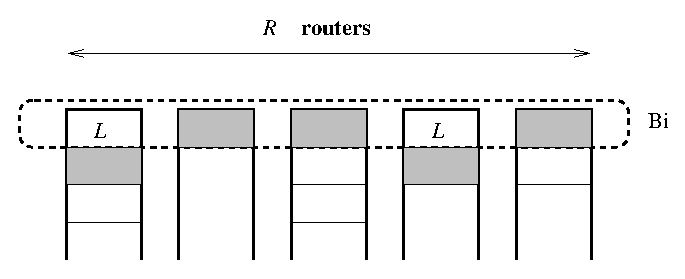
\includegraphics{sandbox/figures/stack2.eps}}
\end{psfrags}
\caption[Implementation of the route computation algorithm from
  Figure~\ref{fig:b2_no_tot_order}.]{Implementation of the route
  computation algorithm from Figure~\ref{fig:b2_no_tot_order}.  Each
  stack represents one of $|R|$ total routers, and each stack element
  represents one of $L$ routes.  The top elements of the $|R|$ stacks
  represent $B_i$, the elements marked $L$ represent routes that are
  worse than the routes at the top of the remaining stacks according
  to the first four steps of the decision process (\ie, local
  preference, AS path length, origin type, MED), and the shaded routes
  represent $B_{i+1}$.  The algorithm terminates when no routes are
  marked $L$.}
\label{fig:b2_stack}
\end{figure}


\textbf{Computational Complexity.}
Understanding the running time of the algorithm in
Figure~\ref{fig:b2_no_tot_order} is easiest when we consider the
implementation of the algorithm shown in
Figure~\ref{fig:b2_stack}.   In this figure, the eBGP-learned routes at
each router are represented as a stack and are sorted {\em locally}
(\ie, compared only to other routes learned at the same router).  The
top of the stack represents the best route learned at that router;
the route that is second from the top is the second best route, and
so forth.  Then, the algorithm from Figure~\ref{fig:b2_no_tot_order}
can be interpreted as follows:
\begin{itemize}
\itemsep=-1pt
\item $B \leftarrow \cup_r \lambda_r(C_r)$ is the union of all of the
  elements at the top of the stack and does not need to be computed
  explicitly, assuming each stack is sorted.  The complexity of sorting
  $N$ routes distributed across $|R|$ stacks is $O(N \log N)$.  Each of
  $N$ routes may be inserted into as many as $|R|$ stacks, so the
  complexity of this step is $O(N \log N + N|R|)$.
\item $L \leftarrow B \setminus \gamma(B)$ marks a route at the top
  of a stack if that route is worse than any route at the top of
  another stack, according to the first four steps of the BGP decision
  process.  This process takes at most two scans of the routes at the
  top of the $|R|$ stacks, so the running time is $O(|R|)$.
\item $C \leftarrow C \setminus L$ ``pops'' the marked routes from the
  top of 
  the stacks, where appropriate.  This process requires a single scan
  through $|R|$ stacks and at most $|R|$ pop operations, so the running time
  is $O(|R|)$.  
\end{itemize}

In the worst case, the above three steps repeat until $N-1$ routes are
popped from the stacks, and each iteration only pops a single route.
Thus, in the worst case, the running time for the algorithm is $O(N \log
N + N|R|)$.


%\begin{theorem}\label{th:noelim_global}
%The second phase of the BGP route prediction algorithm
%, which selects
%the set of best routes at the eBGP-speaking routers, 
%does not backtrack.
%\end{theorem}

%% \noindent
%% The proof of this theorem follows from two proofs in our previous
%% work~\cite{feamster:02}. In this work, we first show that the second
%% phase of the route prediction algorithm never eliminates a candidate
%% route that an eBGP-speaking router would have selected as its best route
%% (Theorem A.4) and the algorithm always eliminates every candidate route
%% that BGP eliminates (Theorem A.4).  Additionally, the second phase of
%% the algorithm correctly predicts the set of best eBGP routes without
%% backtracking.



%%%%%%%%%%%%%%%%%%%%%%%%%%%%%%%%%%%%%%%%%%%%%%%%%%%%%%%%%%%%



\section{Route Computation without Full Visibility}
\label{sec:best_egress}

A full mesh iBGP topology does not scale to large networks because a
network of $|R|$ routers requires $O(|R|^2)$ iBGP sessions.  Network
operators use a technique called {\em route reflection}, which improves
scalability by introducing hierarchy but complicates route prediction.
%
First, we define an iBGP
signaling topology, expound on problems introduced by route reflection,
and
describe constraints on iBGP configuration that must hold for modeling
to be possible. Next, we propose an algorithm that
efficiently computes the outcome of BGP path selection in a network with
route reflection; we then present a minor
modification to the algorithm that is necessary if MED is only compared
across routes from the same neighboring AS.

\subsection{Problems Introduced by Route Reflection}\label{sec:problems_rr}

\begin{figure}
\begin{center}
\begin{psfrags}
\psfrag{RR1}{{\LARGE $RR_1$}}
\psfrag{RR2}{{\LARGE $RR_2$}}
\psfrag{W}{{\LARGE $W$}}
\psfrag{X}{{\LARGE $X$}}
\psfrag{Y}{{\LARGE $Y$}}
\psfrag{Z}{{\LARGE $Z$}}
\resizebox{0.5\linewidth}{!}{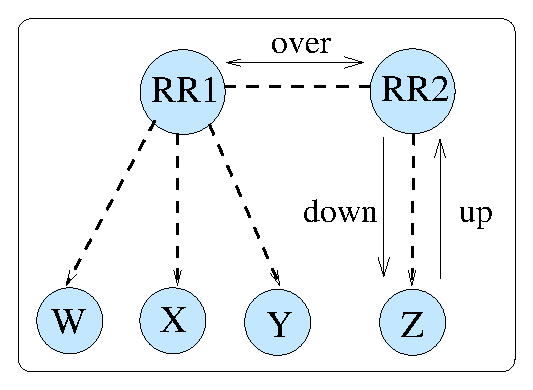
\includegraphics{sandbox/figures/ibgp.eps}}
%\centerline{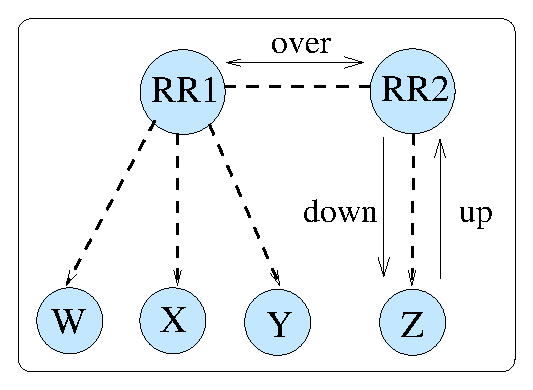
\epsfig{file=sandbox/figures/ibgp.eps,width=0.5\columnwidth}}
\end{psfrags}
\end{center}
\caption{Example iBGP signaling graph.}
\label{fig:ibgp}
\end{figure}


%%%
%%% Signaling graph
%%%
A router does not normally forward iBGP-learned routes over other iBGP
sessions, but it can be configured as a {\em route reflector\/} (RR),
which forwards routes learned from one of its route-reflector clients to
its other clients.  The routers in an AS form a directed graph, $G =
(R,S)$, of iBGP sessions called a {\em signaling graph}. Each edge $a =
(u,v) \in S$ where $u,v \in R$ corresponds to an iBGP session between a
pair of routers. We then define three classes of edges: (1)~$a \in \mbox{{\bf
down}}$ if $v$ is a route-reflector client of $u$; (2)~$a \in \mbox{{\bf
up}}$ if $u$ is a route-reflector client of $v$; and (3)~$a \in
\mbox{{\bf over}}$ if $u$ and $v$ have a regular iBGP session between
them.  Figure~\ref{fig:ibgp} shows an example signaling
graph.  In a full-mesh configuration, every eBGP-speaking router has an edge
in {\bf over} with every other router in the AS, 
and both the {\bf up} and {\bf down} sets are empty. 
%\footnote{Occasionally, routers within an AS can also be grouped
%into ``confederations''; because these are used much less frequently
%than route reflectors, we focus on modeling route reflectors.}



Previous work has shown that iBGP satisfies safety as long as the
structure of the signaling graph satisfies certain sufficient
conditions~\cite{Griffin2002}.  Accordingly, we refine
Constraint~\ref{a:ibgp} in terms of these sufficient conditions to
guarantee that an iBGP topology with route reflection satisfies safety
(at least when the MED attribute is not used or compared across all
routes):

\begin{constraint}
\label{a:sane2}
(1)~$\forall \;u,v,w \in R$, $((u,v) \in \mbox{{\bf down}} \mbox{
  and } (u,w) \not\in \mbox{{\bf down}}) \Rightarrow
  \lambda_u(\{\rho_v,\rho_w\}) = \rho_v$, where $\rho_v$ represents any route
  learned from $v$ and $\rho_w$ is any route from $w$;
%\lambda_r(r_v) >
%\lambda_r(r_w)$
and (2)~the edges in $\mbox{{\bf up}}$ are acyclic.
%, and
%(c) the shortest IGP path between each pair of routers is a valid
%signaling path.
\end{constraint}
\vspace{0.1in}

\noindent
Part (a) is satisfied when routers do not change the attributes of
iBGP-learned routes and each router has a lower IGP path cost to its
clients than to other routers. The common practices of applying import
policies only on eBGP sessions and placing route reflectors and their
clients in 
the same point-of-presence (\ie, ``PoP'') ensure that these
conditions hold.
%
Part (b) states that if $a$ is a route reflector for $b$, and $b$ is a
route reflector for $c$, then 
$c$ is not a route reflector for $a$, consistent with the notion of a
route-reflector {\em hierarchy} (rather than an arbitrary signaling graph).  


%%%
%%% Convergence to a single answer
%%%
Even a route reflector configuration that converges can wreak havoc on
the algorithms from Sections~\ref{sec:simple} and~\ref{sec:med_model}.
A route reflector hides information by advertising only a {\em single
best route to its iBGP neighbors}.
For example, in
Figure~\ref{fig:ibgp}, if $W$ and $Z$ have eBGP-learned routes, router
$Y$ learns a single route from its route reflector $RR_1$.  Suppose that
$RR_1$ selects the eBGP route advertised by $Z$.
Then, $Y$ would pick $Z$'s route as well,
even if $Y$ would have preferred $W$'s route over $Z$'s route.  Note
that $Y$ 
makes a different routing decision than it would if it could select
its best route from all the eBGP routes (\ie, from both $W$ and $Z$).
In large networks, route reflection reduces the number of routing
messages and iBGP sessions, which helps scalability, but it complicates
route prediction in the following ways:

\begin{enumerate}
\itemsep=-1pt

\item A router will not typically learn every route that is equally good
  up through the first four steps of the decision process.  That is, it
  is possible (and likely) that some routers will not learn every route
  in $\gamma(B)$.  In Section~\ref{sec:rr_nomed}, we describe an
  algorithm that handles this case.
%  This fact is significant because the route computation algorithm
%  cannot elimiante a route simply because it is not in $\gamma(B)$ (as
%  in Figure~\ref{fig:b2_no_tot_order} Section~\ref{sec:fm_med}).

\item If a network uses route reflectors, {\em and} MED is only
  compared across routes from the same AS, the routes that some routers
  ultimately select may be {\em worse} than some
  eBGP-learned routes, according to the first four steps of the
  decision process.  That is, it may be the case that $b_r \not\in
  \gamma(E)$ for some router $r$.  This characteristic 
  creates problems not only for efficient route prediction, but also for
  safety. 
  We discuss this case in Section~\ref{sec:rr_med}.
%This artifact is significant because
%  the algorithm can no longer eliminate a candidate route simply because
%  it is not contained in $\gamma(E)$.
\end{enumerate}

\subsection{Algorithm: Route Reflection, No MED}\label{sec:rr_nomed}

Route reflection obviates the need for routers in an AS to form a full
mesh topology, but it also means that some routers may not learn all
routes in $\gamma(B)$.  This artifact has two implications.  First, the
algorithm cannot simply assign a non-eBGP-speaking router the route from
the ``closest'' eBGP-speaking router, because the former router may
never learn the route.
% corresponding to the shortest path to the exit.
Thus, applying $b_r \leftarrow \lambda_r(B)$ may not always be
correct. 
%Rather, the routing alternatives
%available to a particular router depends on its position in the route
%reflector hierarchy. 
%
For example, consider the network shown in Figure~\ref{fig:ibgp1}.  $W$,
$X$, and $Y$ are clients of route reflector $RR$, and $Z$ is a regular
iBGP peer of $Y$.  $X$ and $Y$ have a short IGP path between them, but
they are {\em not} directly connected by an iBGP session.  Routers $W$,
$X$, and $Z$ have eBGP routes that are equally good through the first
four steps of the route selection process, and have thus selected their own
eBGP-learned routes.  In this network, $Y$'s closest egress point is
$X$, but $Y$ selects $W$, because $RR$'s closest egress router is $W$.
%

Second, often there is {\em no consistent ranking of possible egress
  routers} from some non-eBGP-speaking router; in other words, {\em
  egress determinism} (Definition~\ref{def:egress_determinism}) is
  violated. 
%
For example, in Figure~\ref{fig:ibgp1}, 
$RR$ prefers egress router $W$
because its IGP path 
cost to $W$ is the shortest.  Router $Y$'s preferences over possible egress
routes depends on the presence or absence of other routes.  If the AS
learns routes for some destination via eBGP sessions at routers $X$ and
$Z$, then router $Y$ prefers using $X$ as an egress router.  On the
other hand, if the AS learned routes at $W$, $X$, and $Z$, then $Y$
prefers using $Z$, which implies that $Y$ prefers egress $Z$ over $X$
and is inconsistent with $Y$'s choice when only $X$ and $Z$ are
available egress routers.

\begin{figure}[t]
\begin{center}
\begin{psfrags}
\psfrag{RR}{{\LARGE $RR$}}
\psfrag{W}{{\LARGE $W$}}
\psfrag{X}{{\LARGE $X$}}
\psfrag{Y}{{\LARGE $Y$}}
\psfrag{Z}{{\LARGE $Z$}}
\resizebox{0.5\linewidth}{!}{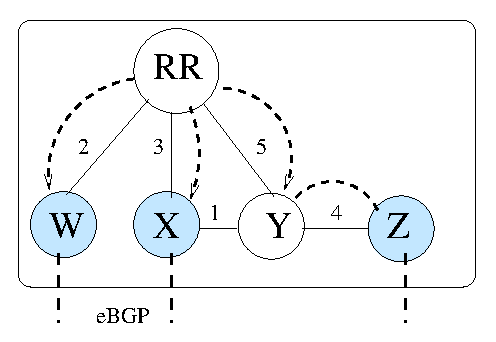
\includegraphics{sandbox/figures/ibgp1.eps}}
\end{psfrags}
\end{center}
\caption{When an AS's iBGP topology uses route reflectors, a router may
  not always discover the route corresponding to its closest egress
  router. }
\label{fig:ibgp1}
\end{figure}

\begin{figure}[t]
\begin{small}
\begin{center}
\centering{\em Algorithm: Route Reflection, No MED} \\
\centering\framebox{
\begin{minipage}{4in}
\begin{tabbing}
\hspace*{0.5cm}\=\hspace{0.5cm}\=\hspace{0.5cm}\=\hspace{0.3cm}\=
\hspace{0.3cm}\=\hspace{0.3cm}\=\hspace{0.3cm}\=\hspace{0.3cm}\=\kill
{\sc SelectBest\_eBGP\_RR}($E$, $R$)\\
%\> {\em Build sets containing the top and bottom of the graph.} \\
%\> $T \leftarrow \{ r | r \in R \mbox{and} \not\exists s \; \mbox{s.t.}
%(r,s) \in \mbox{{\bf up}} \}$ \\
%\> $M \leftarrow \{ r | r \in R \mbox{and} \not\exists s \; \mbox{s.t.}
%(r,s) \in \mbox{{\bf down}} \}$ \\
%\\
%\> {\em Mark bottom as activated and assign best routes.}\\
%\> $A \leftarrow M$\\
%\> $B \leftarrow \cup_r\lambda_r(E_r)$ \\
%\\
\\
\> {\em // Proceed up the hierarchy, assigning best routes.} \\
\> {\em // Find a router for which all children are activated.} \\
\> $A \leftarrow \phi$\\
\> {\bf while} $\exists r \in R$ s.t. $r \not\in A$ and $c
\in A \; \forall c \in \mbox{{\sc down}}(r)$\\ 
\>\> $I_r \leftarrow \cup_{c \in\mbox{{\sc down}}(r)} b_c$ \\
\>\> $b_r \leftarrow \lambda_r(I_r \cup E_r)$ \\
\>\> $A \leftarrow A \cup r$ \\
\\
\> {\em // Proceed down the hierarchy.} \\
\> {\em // Find a router for which all parents are activated.} \\
\> $A \leftarrow \phi$\\
\> {\bf while} $\exists r \in R$ s.t. $r \not\in A$ and $c
\in A \; \forall c \in \mbox{{\sc up}}(r)$\\ 
\>\> $I_r \leftarrow \cup_{c \in\mbox{{\sc up}}(r) \cup \mbox{{\sc
      over}}(r)} b_c$ \\ 
\>\> $b_r \leftarrow \lambda_r(I_r \cup b_r)$ \\
\>\> $A \leftarrow A \cup r$ 
\end{tabbing}
\end{minipage}
}
\end{center}
\end{small}
\caption[Algorithm: Route Reflection, No MED]{Algorithm for computing the
  best route at each router in a 
  network with route reflection but no MED.}
\label{fig:best_ibgp}
\end{figure}

To account for the fact that some routes are not visible at some routers,
we design an algorithm that emulates a certain activation sequence,
making route assignments at each router where possible and 
propagating the effects of these decisions to other routers, without
ever having to revisit any assignment. This algorithm is
shown in Figure~\ref{fig:best_ibgp}.
%
The algorithm first activates the routers from the bottom of the
route reflector hierarchy upwards, which guarantees that
each router selects a {\em down\/} route where possible, as
required by Constraint~\ref{a:sane2}(a).   Because the algorithm moves
upwards from the bottom of the hierarchy, it performs computations for
each route reflector after all of the routes from its clients become known;
computations for these routers never need to be revisited, since, by
Constraint~\ref{a:sane2}, a router always prefers routes from its
``children'' (\ie, clients) over routes from its peers or parents.
%
Visiting the routers in the {\em down\/} direction ensures
that the algorithm performs computations for the remaining routers using
all available routes from the {\bf up} and {\bf over} sets.
%Considering the routers in this particular ordering guarantees that no
%router makes a decision that should change later, after some other
%router makes a decision.
%
The algorithm defines two partial orderings of the
routers based on the elements of the {\bf up} and {\bf down} sets.
We can define these two partial orderings because Constraint~\ref{a:sane2}(b)
requires that the signaling graph does not have any cycles of these
edges, so each partial ordering must have a top and bottom element.
%

Applying this algorithm to the example in Figure~\ref{fig:ibgp1}, the
shaded routers select best routes in the first step, because each of those
routers is at the bottom of the hierarchy and, thus, all of their
neighbors in {\bf down} have been activated (because they have none). $Y$
is activated, but it does not select a route at this point because it 
has no neighbors in {\bf down}. 
Because these four routers are at the same level in the hierarchy,
they can be activated in any order.
%
Then $RR$ is activated; it applies $\lambda_{RR}(\{r_W,r_X\})$ and
selects $r_W$ because it has the smallest IGP path cost.  The routers
are all activated again in the downward direction; $Y$ receives $r_W$
from $RR$ and compares it with $r_Z$, which is its best route to the
destination.  $X$ and $Z$ also receive $r_W$ but continue to select
their own route, because $\lambda_r$ prefers eBGP routes over iBGP routes.
We now prove that the algorithm shown in Figure~\ref{fig:best_ibgp} is
correct. 

\begin{theorem}\label{t:exit}
If each router can form a total ordering over the set of all candidate
routes, then the algorithm in Figure~\ref{fig:best_ibgp} correctly
computes the outcome of the BGP decision process, $b_r$, for all routers
$r \in R$.
\end{theorem}
\vspace*{0.1in}

\begin{proof}
Assume that some router $r$ selects a route,
$b_r$, that is different from the route assigned by the algorithm in
Figure~\ref{fig:best_ibgp}, $b'_r$.  
The mismatch can occur in one of two cases: (1)~when $b_r$ 
is learned from a session in {\bf down}, or (2)~when $b_r$ is learned from a
session not in {\bf down} (\ie, in either {\bf up} or {\bf over}).  

Consider Case~1, where $b_r$ is learned from a session in {\bf down}.
Call $b'_r$ the first case of an incorrect computation (\ie, the
algorithm has correctly computed the best route for all routers below
$r$ in the hierarchy); because we examine the first such mismatch, $I_r$
is correct.  If $b'_r$ is also in {\bf down}, then $b'_r = \lambda_r(I_r
\cup E_r)$ when the algorithm proceeds up the hierarchy, which implies
that $b'_r$ is better than $b_r$ according to the BGP decision process,
and $r$ would have actually selected $b'_r$.  If $b'_r$ is in {\bf up}
or {\bf over}, then it must have been the case that it was better,
according to the BGP decision process, than the displaced route $b_r$ in
{\bf down}.
%But then, the algorithm would have also selected $b_r$ using
%$\lambda_r$.
But then, by definition of $\lambda_r$, router $r$ would have also selected
$b'_r$ in BGP.
Thus, the algorithm
correctly computes $b_r$ for all routers $r$ that select a best route
from {\bf down}.


Consider Case~2, where $b_r$ is learned from a session in {\bf up} or
{\bf over}.
%
From the first half of the proof, we know that the algorithm correctly
computes $b_r$ for all routers that 
select a route from {\bf down}, so call $b'_r$ the first instance of a
mismatch for some router that selects a best route from {\bf
up} or {\bf over} (\ie, the algorithm correctly assigns $b_r$ for all
routers higher in the hierarchy than $r$). Again, because we consider the first
such mismatch, we know that $I_r$ is correct. 
%
If 
the route that the algorithm selects, $b'_r$, is in {\bf down}, then, by
Constraint~\ref{a:sane2}(a), BGP could not have selected $b_r$, so we
have a contradiction.  
%
If both $b_r$ and $b'_r$ are learned from
sessions in {\bf up} and {\bf over}, then both are in $I_r$, and,
according to the $\lambda_r(I_r \cup b_r)$ step in the algorithm and by
definition of $\lambda_r$, both the algorithm and the BGP decision
process would select the same route.
\end{proof}

This theorem relates to one from earlier work~\cite{Gao2001a} on
sufficient conditions for stable BGP routing {\em at the AS level}; this
work provides a constructive proof showing that the sufficient
conditions guarantee safety.  In subsequent work, Griffin {\em et
al.} discovered that the sufficient conditions for stable eBGP routing
were analogous to those for stable iBGP routing with route
reflection~\cite{Griffin2002}.  The algorithm from this section applies
the iBGP analog of the constructive proof from the work on stable
interdomain routing to develop an algorithm for {\em computing} that
stable path assignment.

\begin{figure}[t]
\begin{center}
\begin{psfrags}
\psfrag{s}{$s_l$}
\hspace{0.3in}
\resizebox{0.65\linewidth}{!}{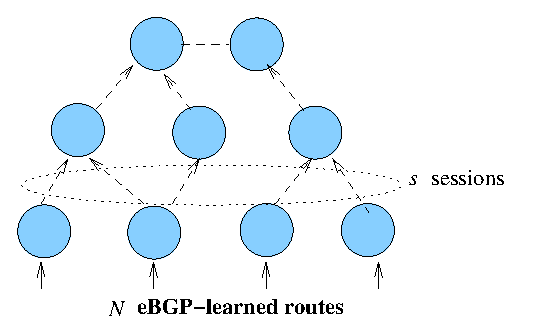
\includegraphics{sandbox/figures/rr_hierarchy.eps}}
\end{psfrags}
\end{center}
\caption[Running time analysis of an iBGP graph walk.]{Running time
  analysis of an iBGP graph walk for the algorithm 
  in Figure~\ref{fig:best_ibgp}.}
\label{fig:rr_hierarchy}
\end{figure}


\textbf{Computational Complexity.}  This algorithm traverses the route
reflector hierarchy exactly twice.  The running time of this algorithm
is $O(N + |S|)$, where $N$ is the number of eBGP-learned routes, and
$|S|$ is the number of iBGP sessions.  To see why this is the case,
consider the $l$-level route reflector hierarchy pictured in
Figure~\ref{fig:rr_hierarchy}.  Starting from the bottom of the
hierarchy, the algorithm must perform comparisons over $N$ routes to
determine the routes that the $M$ routers at the bottom of the hierarchy
select (the number of routers at the bottom of the hierarchy is
inconsequential: these comparisons can be performed by constructing a
subset of $M$ routes from the original $N$ routes, which can be
performed in a single scan of the $N$ routes).  The algorithm then
propagates the selection of these $M$ routes to the next level of the
hierarchy, where $s_l$ comparisons must be performed across the routers
at the next highest level, where $s_l$ is the number of iBGP sessions at
level $l$.  Repeating this process up the hierarchy yields a total
running time of $O(N+|S|)$.

Recall from Section~\ref{sec:simple} that the running time for
the algorithm in the case of full-mesh iBGP, was $O(N+|R|^2)$, or
$O(N+|S|)$.  Note that the algorithm for the case with route reflection
has the {\em same} running time complexity as before; the running time
for computing the outcome of BGP route selection is no more complex,
even though the process for computing the outcome is more involved.
In an iBGP topology with route reflection, the number of sessions,
$|S|$, will actually be less than $|R|^2$; thus, the running time of the
algorithm benefits from the fact that route reflectors
reduce the number of sessions in the iBGP topology.


%\subsection{Route Prediction with Route Reflection and MED}

\subsection{Algorithm: Route Reflection, MED}\label{sec:rr_med}

When a network uses both route reflection and MED, the graph walk
algorithm in Figure~\ref{fig:best_ibgp} no longer works, because it
relies on the fact that all routers will ultimately
select a route in $\gamma(E)$.  In a network with route reflection {\em
and} MED, this is not always true, because when a router selects a
locally best route, a route with a lower MED value might not be visible
to that router.  As a result, some router in the AS might select an
eBGP-learned route that is {\em worse}, according to the first four
steps of the BGP route selection process, than eBGP-learned routes
selected by other routers!  Figure~\ref{fig:ibgp3} shows an example of
exactly this scenario.

\begin{figure}[t]
\begin{center}
\subfigure[When $Y$ is closer to $RR$ than $X$, the routing system
  satisfies safety.]{
\begin{psfrags}
\psfrag{a}{{\Large $a$}}
\psfrag{b}{{\Large $b$}}
\psfrag{c}{{\Large $c$}}
\psfrag{d}{{\Large $d$}}
\psfrag{RR}{{\LARGE $RR$}}
\psfrag{W}{{\LARGE $W$}}
\psfrag{X}{{\LARGE $X$}}
\psfrag{Y}{{\LARGE $Y$}}
\psfrag{Z}{{\LARGE $Z$}}
\resizebox{0.45\linewidth}{!}{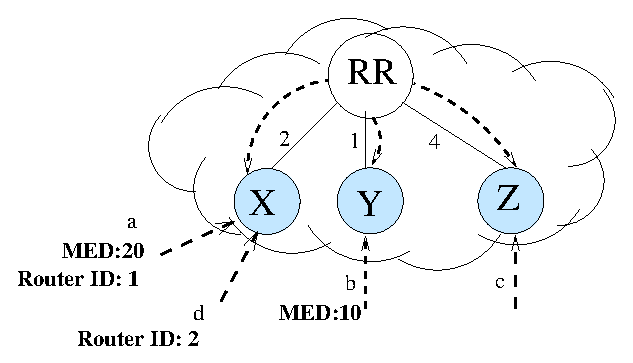
\includegraphics{sandbox/figures/ibgp3.eps}}
\end{psfrags}
}\hfill
%
\subfigure[When $X$ is closer to $RR$ than $Y$, the routing system
  violates safety and the algorithm in Figure~\ref{fig:best_ibgp} is
  incorrect.]{ 
\begin{psfrags}
\psfrag{a}{{\Large $a$}}
\psfrag{b}{{\Large $b$}}
\psfrag{c}{{\Large $c$}}
\psfrag{d}{{\Large $d$}}
\psfrag{RR}{{\LARGE $RR$}}
\psfrag{W}{{\LARGE $W$}}
\psfrag{X}{{\LARGE $X$}}
\psfrag{Y}{{\LARGE $Y$}}
\psfrag{Z}{{\LARGE $Z$}}
\resizebox{0.45\linewidth}{!}{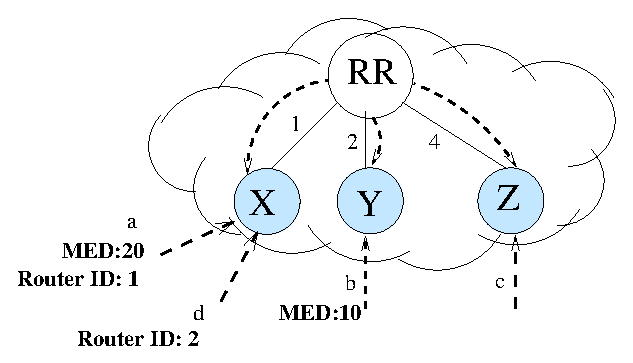
\includegraphics{sandbox/figures/ibgp3b.eps}}
\end{psfrags}
}
\end{center}
\caption[An example where the algorithm in
  Figure~\ref{fig:best_ibgp} produces the incorrect result.]{A BGP
  configuration where the algorithm in Figure~\ref{fig:best_ibgp}
  may the incorrect result, depending on the IGP topology and the MED
  attributes of the routes received via eBGP.}
\label{fig:ibgp3}
\end{figure}

Note that applying the algorithm from Figure~\ref{fig:best_ibgp} does
not always correctly compute the outcome of the BGP decision process.
Consider the operation of the algorithm from Figure~\ref{fig:best_ibgp}
on the topology and route announcements shown in Figure~\ref{fig:ibgp3}(a).
Proceeding up the hierarchy: (1)~routers $X$, $Y$, and $Z$ would select
routes $a$, $b$, and $c$, respectively; (2)~$RR$ selects route $b$
because $b$ has a lower MED value than $a$ and a shorter IGP path to the
egress than $c$.  Proceeding down the hierarchy, $X$ selects $b$ because
it has a lower MED value than $a$.  At this point, the algorithm in
Figure~\ref{fig:best_ibgp} would terminate in the case of
Figure~\ref{fig:ibgp3}(a), but, in fact, depending on the IGP topology
$X$'s selection of $d$ could have caused $RR$ to select a new best
route.  Suppose, instead, that the IGP topology were such that $RR$ were
closer to $X$ than to $Y$, as in Figure~\ref{fig:ibgp3}(b).  In this
case, proceeding up the route reflector hierarchy a second time would
cause $RR$ to change its selected route from $b$ to $d$; subsequently
proceeding down the hierarchy would cause $X$ to change its selected
route from $d$ to $a$.  In fact, as described in a similar example in
Section~\ref{sec:safety_def}, BGP does not satisfy safety in this
example---therefore, {\em no} number of progressions up and down the
iBGP hierarchy would cause the algorithm to predict the correct outcome.


%% In Figure~\ref{fig:ibgp2},
%%  $X$ would learn routes $a$ and $c$, rather than $a$ and $b$,
%% and it would ultimately select $b$, because it never learns route $b$,
%%  which has a lower MED value than route $a$.  
%% If,
%% however, as shown in Figure~\ref{fig:ibgp3}, $X$ had learned a second
%% eBGP-learned route, $d$, that was {\em better} than $b$ (because it was
%% learned via eBGP), but worse than $a$ (due to router ID), then $X$ would
%% ultimately select $d$, which is an eBGP-learned route but {\em not} its
%% locally best eBGP route, and not even in $\gamma(E)$.


In this situation, any router in the AS might ultimately select a route
that is not in $\gamma(E)$; as a result, the route prediction algorithm
cannot eliminate a route from the set of candidate routes $C_r$ at any
router $r$, as was done in the case where determinism did not hold but
every router was guaranteed to learn every eBGP-learned route
(Section~\ref{sec:med_model}, Figure~\ref{fig:b2_no_tot_order}).  As we
have seen, the fact that a router may select a route that is not in
$\gamma(E)$ as its best route, the algorithm (and BGP route selection,
for that matter) is no longer guaranteed to terminate.  
%% In fact, the
%% fact that the algorithm may not terminate is consistent with the
%% observation that even very simple iBGP route reflector configurations
%% where MED is only compared across routes from the same AS {\em may not
%% converge at all} (see Section~\ref{sec:safety_def},
%% Example~\ref{ex:med_det}).

It might initially seem reasonable to impose constraints on the iBGP and
IGP topologies that guarantee safety and can easily be checked with a
tool like \rcc (Chapter~\ref{chap:rcc}).  Unfortunately, as the
example in Figure~\ref{fig:ibgp3}
shows, any condition that guarantees safety would require knowledge of
the MED attributes of every eBGP-learned route to a destination, not
just the iBGP and IGP topologies.  Further, the simplicity of this
example demonstrates that any condition that guarantees safety for any
combination of eBGP routes would be overly restrictive (\ie, it would
essentially require not using route reflectors).  Thus, in the case
where a BGP configuration uses route reflection and only compares the
MED attribute across routes from the same AS, the most efficient
algorithm for determining the outcome of BGP route selection (and
detecting safety violations) is actually a simulator.  In other words,
there are no conditions on the topology that can be enforced to
guarantee that an algorithm would never have to visit each router in the
AS more than once, or even that BGP would satisfy safety.
